\section{Systemets funktionelle krav}

Systemet har til formål at hjælpe apopleksipatienter med rehabiliteringen af deres balancefunktion i hjemmet. Dette gøres ved en træningøvelse, hvor systemet skal gå ind og advare patienten om risiko for fald under øvelsen. Måden patienten skal advares, er ved at måle kropshældningen under forsøget. Hvis patienten kommer til at hælde for meget, skal der være et biofeedback system, som advarer patienten om hvilken retning de er ved at falde til højre eller venstre. Feedbacksystemet udgøres af en visuel og en sensorisk del. %Der benyttes to feedback dele, da brugeren af systemet kan være dårligt seende, eller have kognitive problemer, som kan gøre det svært at opfange kun en form for feedback.   
Derudover skal der være en digital feedback, som kan gemmes, så øvelsens resultater kan ses igen. 

De funktionelle krav:
\begin{itemize}
\item Kunne anvendes i hjemmet af apopleksipatienter
\item Måle kropshældning
\item Give visuel og sensorisk feedback
\item Give digital feedback
\end{itemize}

\section{Systemets opbygning}
\begin{figure}[H]
\centering
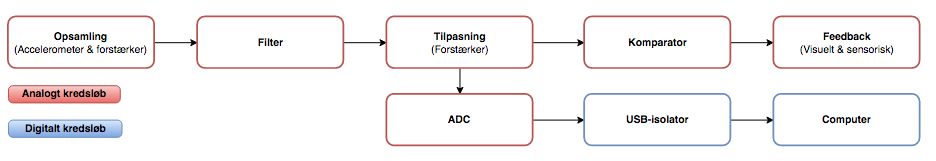
\includegraphics[scale=0.5]{figures/Blokdiagram.jpg}
\caption{Her ses et blokdiagram af systemets opbygning}
\label{Blokdiagram}
\end{figure}